% !TEX encoding = UTF-8
% !TEX program = xelatex
\documentclass[12pt,a4paper]{article}
\usepackage[paperwidth=210mm, paperheight=297mm, left=0.75in, right=0.75in, bottom=1in, top=1in]{geometry}
%\usepackage{geometry}
\usepackage{polyglossia}
\setdefaultlanguage[babelshorthands]{italian}
\usepackage{fontspec}
%\usepackage{cite}
\usepackage{graphicx}
%\usepackage[fixlanguage]{babelbib}
%\selectbiblanguage{italian}
\usepackage{blindtext}
\usepackage{wrapfig}

\frenchspacing
\makeindex

\begin{document}
\title{\vspace{-70pt}OAO 2}
\author{Chiara Bettinelli}
\date{}
\maketitle
\pagestyle{empty}
\thispagestyle{empty}

\section*{Storia}
\label{storia}
\begin{wrapfigure}{r}{0.35\textwidth}
  \vspace{-10pt}
  \begin{center}
    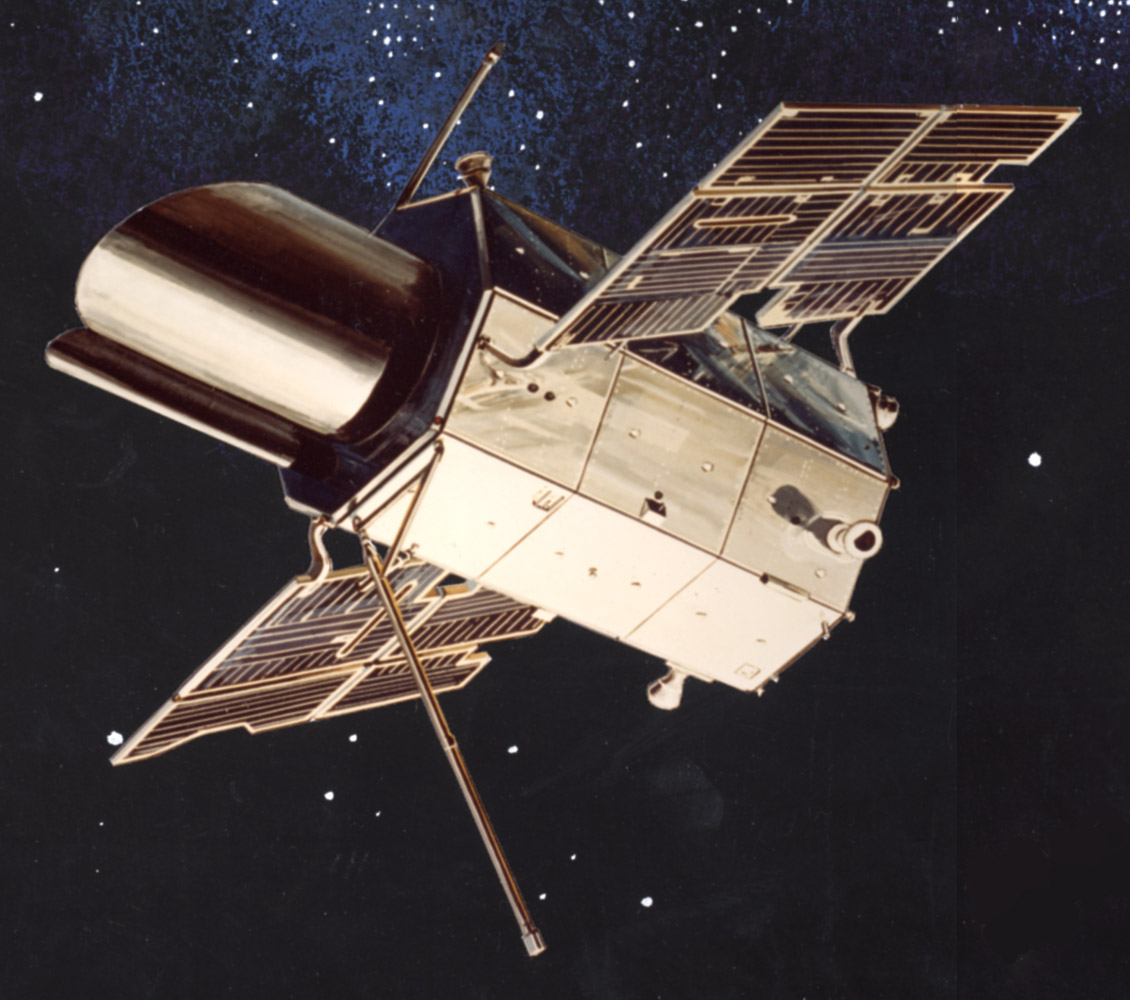
\includegraphics[width=0.30\textwidth]{satellite}
  \end{center}
  \vspace{-20pt}
  %\caption{A gull}
\end{wrapfigure}
L'OAO 2 fu lanciato il \textbf{7 dicembre 1968} con un razzo vettore Atlas-Centaur da Cape Canaveral Air Force Station. Il satellite aveva 11 telescopi per le osservazioni nell'ultravioletto e restò in funzione fino al gennaio 1973. L'OAO 2 è stato uno di una serie di osservatori astronomici automatici.

\section*{Osservazioni}
\label{osservazioni}

L'OAO 2, noto anche come \textbf{Stargazer}, permise di scoprire che le comete sono circondate da un enorme alone di idrogeno che si estende per centinaia di migliaia di chilometri; inoltre effettuò osservazioni su \textbf{stelle novae} in luce ultravioletta.

\section*{Curiosità}
\label{curiosit}

Il programma Orbiting Astronomical Observatory (OAO) (in italiano Osservatorio Astronomico Orbitante) era basato su una famiglia di quattro satelliti artificiali che dovevano essere lanciati dalla NASA tra il 1966 e il 1972. Essi dovevano effettuare le prime osservazioni in alta risoluzione di numerosi oggetti nella banda dell'ultravioletto. Anche se due missioni fallirono, il successo delle altre due fece prendere coscienza alla comunità degli astronomi dei benefici degli osservatori spaziali e condusse in seguito alla creazione del telescopio spaziale Hubble.
\end{document}


\end{document}